% IMPLEMENTATION

% - introduction
In this chapter, details on implementation of the proposed method are discussed. Code is listed in Appendix \ref{app:code}, supplied on DVD, and made available online\footnote{Code available on Google Code: http://code.google.com/p/martijn-msc-thesis}; this chapter will complement the code and will serve as a general introduction, therefore no code is listed in this chapter. The pipeline given in Section \ref{pipeline} will be used as a guideline, allowing the reader to follow the process in execution order. This order, though, is not necessarily the order of implementation; in fact, most applications developed for visualisation (last step in the pipeline) were written in an early stage, allowing for following progress and viewing intermediate steps. Developing geometry reconstruction algorithms greatly benefits from the ability to quickly shoot footage, run suggested and implemented algorithms, \emph{visualise} intermediate steps, and suggesting modified algorithms. Details on collecting datasets (first step in the pipeline) are discussed in the next chapter; implementation details of the remaining steps in the pipeline are discussed after an overview of the libraries that are being used.


% - libraries and external code
\section{Libraries}  \label{libraries}
All tools are written using platform-independent and open-source libraries, and all code should compile and run on all major platforms (although extensive tests have only been done under Linux, Ubuntu 12.04). The same holds for all tested external tools (SfM step), except Voodoo which is only free for research-purposes. All tools developed for this thesis are written in C++ and a cmake config file is provided.

The well-established computer vision library \textbf{OpenCV}\footnote{OpenCV homepage: http://opencv.willowgarage.com} \OpenCV is used for general image and video i/o, and 2D image and feature visualisation. Very recently, a sister project called \textbf{Point Cloud Library}\footnote{PCL homepage: http://pointclouds.org} (PCL) was announced by \Rusu2011, providing common data structures, algorithms, and tools useful for 3D computer vision. Although PCL still lacks extensive documentation and has a rapidly changing API, it does provide useful data structures and tools for handling point clouds, including advanced filter, segmentation and surface algorithms. Regrettably, it has (yet) no data structures for visibility information nor a commonly-agreed camera representation, reflecting the rare interest in visibility and occlusion (Sect. \ref{sfm}), so they have been developed for this thesis. In addition, the provided voxel grid representations are mostly useful for space partitioning and searching. Instead, we used the more suitable and feature-rich library \textbf{OctoMap}\footnote{OctoMap homepage: http://octomap.sourceforge.net}, recently released by \Wurm2010. OctoMap was chosen because it makes use of probabilistic nodes, implements a memory-efficient octree instead of same-size voxels, and allows for ray shooting. It also includes an octree viewer. Lastly, a set of open-source C++ files released by \Boykov2004 has been used for efficient graph-cut regularisation. Needless to say, writing methods to convert between representations of these four libraries was inevitable.


% - pipeline:
\section{Pipeline implementation}  \label{pipeline-implementation}

%   - SfM tools
\subsection{Structure from Motion}
Camera models and a feature point cloud can be obtained by standard Structure from Motion algorithms (Sect. \ref{sfm}). Structure from Motion has been implemented oftentimes already. Nowadays, reliable software tools are available for processing image sequences and outputting camera poses and point clouds. Both commercial and open-source tools exist. Since the proposed algorithms use SfM output as is and do not innovate on the SfM process itself, we experimented with three freely available Structure from Motion tools instead of building our own. The tools tested are Bundler, Voodoo, and VisualSfM. All tools are used with default settings.

Originating as part of the Photo Tourism work \cite{Snavely2006} and released under the GPL open-source license, \textbf{Bundler}\footnote{Bundler homepage: http://phototour.cs.washington.edu/bundler} became an authority and is still one of the most cited SfM systems. Originally developed for unordered photo collections taken from the internet, it claims to work on normal sequences too. The command line tool takes a directory with images as input, extracts and matches SIFT features and descriptors by default, and optimises estimated parameters incrementally using sparse bundle adjustment. Bundler outputs an ASCII file containing camera models, triangulated points with colours and visibility lists. The latest binary version (0.3) was tested.

\textbf{Voodoo}\footnote{Voodoo homepage: http://www.digilab.uni-hannover.de/docs/manual.html} was developed as non-commercial alternative to software tools such as Boujou and is free to use for research purposes. Finding and matching SIFT descriptors is possible, although by default Harris edge detection is used and points are tracked over the sequence. Voodoo is developed for sequences only for which the small displacement assumption is reasonable. The GUI allows for manually fine-tuning of estimated feature tracks (\eg linking a lost feature point to its rediscovery a few frames later) and includes simple modelling tools for improving the results, but those are not used during testing. Voodoo outputs various ASCII file formats, but unfortunately none of them includes visibility information. The latest version (1.2.0 beta) was tested.

Recently, a new graphical tool called \textbf{VisualSfM}\footnote{VisualSfM homepage: http://www.cs.washington.edu/homes/ccwu/vsfm/} by \Wu2011 was released that constitutes a graphical shell around a GPU implementation of both SIFT (SiftGPU) and Bundle Adjustment by \Wu2011 for SfM, and the CMVS/PMVS tools by \Furukawa2010 for patch-based dense multi-view stereo. VisualSfM and its components are all released under the GPL license. VisualSfM outputs an ASCII file similar to Bundler's format, and a binary file after the optional dense reconstruction step. The interface offers visual feedback during incremental bundle adjustment, and provides quite a few other useful visualisations. The latest version (0.5.17) was tested.

Example outputs are shown for two datasets; one example frame for each is pictured in Fig. \ref{fig:sfmcomparison0}). The chess dataset gives typical results and are shown in Figure \ref{fig:sfmcomparison1}; good results are obtained for the houses1 dataset, shown in Figure \ref{fig:sfmcomparison2}. More details on all datasets used in this thesis are listed in Appendix \ref{app:datasets}.

In general, Bundler performs poorly on the supplied datasets. Output usually consists of a point cloud without identifiable structures. An explanation for the bad results can lie in the fact that Bundler is developed for unordered sequences and therefore uses no prior for camera displacement nor for possible identical camera models. Indeed, estimated camera locations often have a variety of distances (and intrinsics) from the point cloud, where the other two tools place cameras in a string. Voodoo often exports reasonable results with, indeed, trustworthy looking camera paths and point clouds. It does not export colours and does not automatically rediscover points lost during tracking earlier on in the sequence, and no bundle adjustment is used to improve results. Using SIFT matching does not improve results, and matching only occurs between nearby frames. Voodoo results often contain a fair amount of points triangulated very far away from the scene. More importantly, none of the variety of export formats contains visibility lists. VisualSfM gives good results on almost all tested sequences. Due to its GPU implementation, it is faster than Bundler (and Voodoo in SIFT matching mode): two hours on sequences of 500 frames against half a night. Visual feedback during reconstruction and bundle adjustment is useful for monitoring progress. Due to Bundler's bad results, Voodoo's lack of visibility lists, and VisualSfM's good performance over all, VisualSfM is used for all further experiments.

\begin{figure}[htb!]
 \centering
 \subfigure[Frame 70 of chess dataset]{
  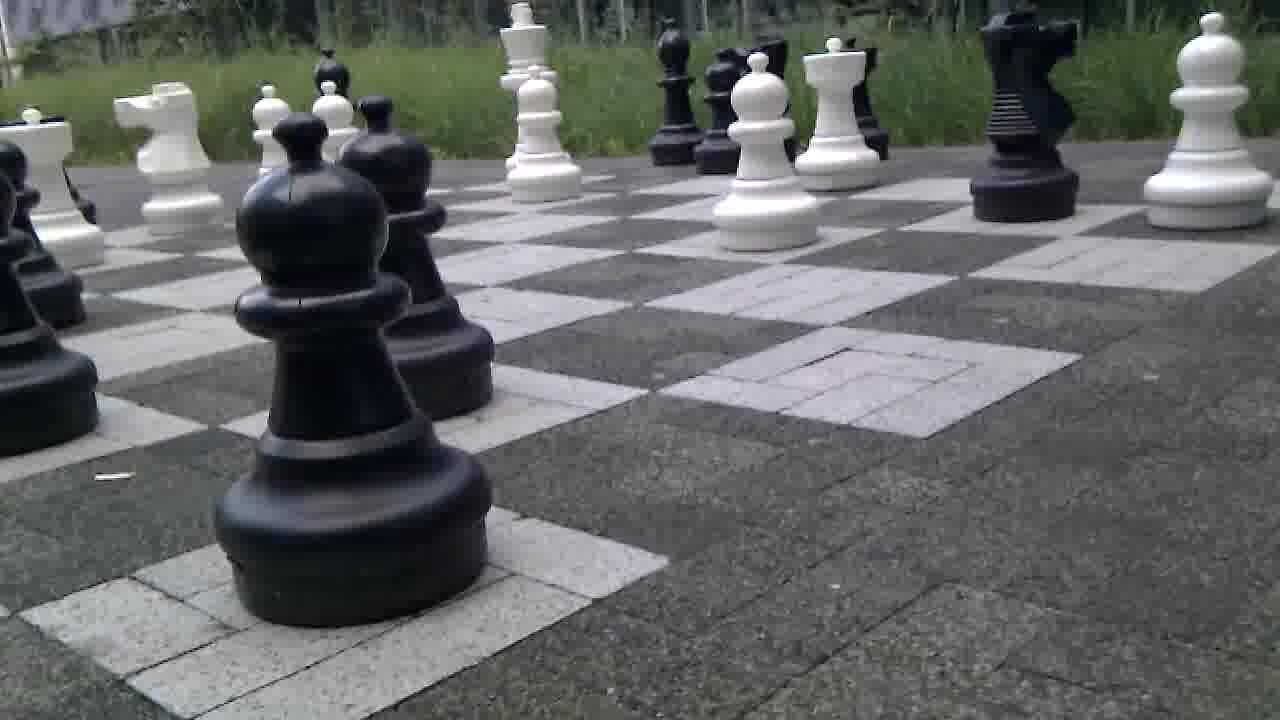
\includegraphics[width=0.55\textwidth]{img/chess_frame70}  \label{fig:}
 }
 \subfigure[Frame 11 of houses1 dataset]{
  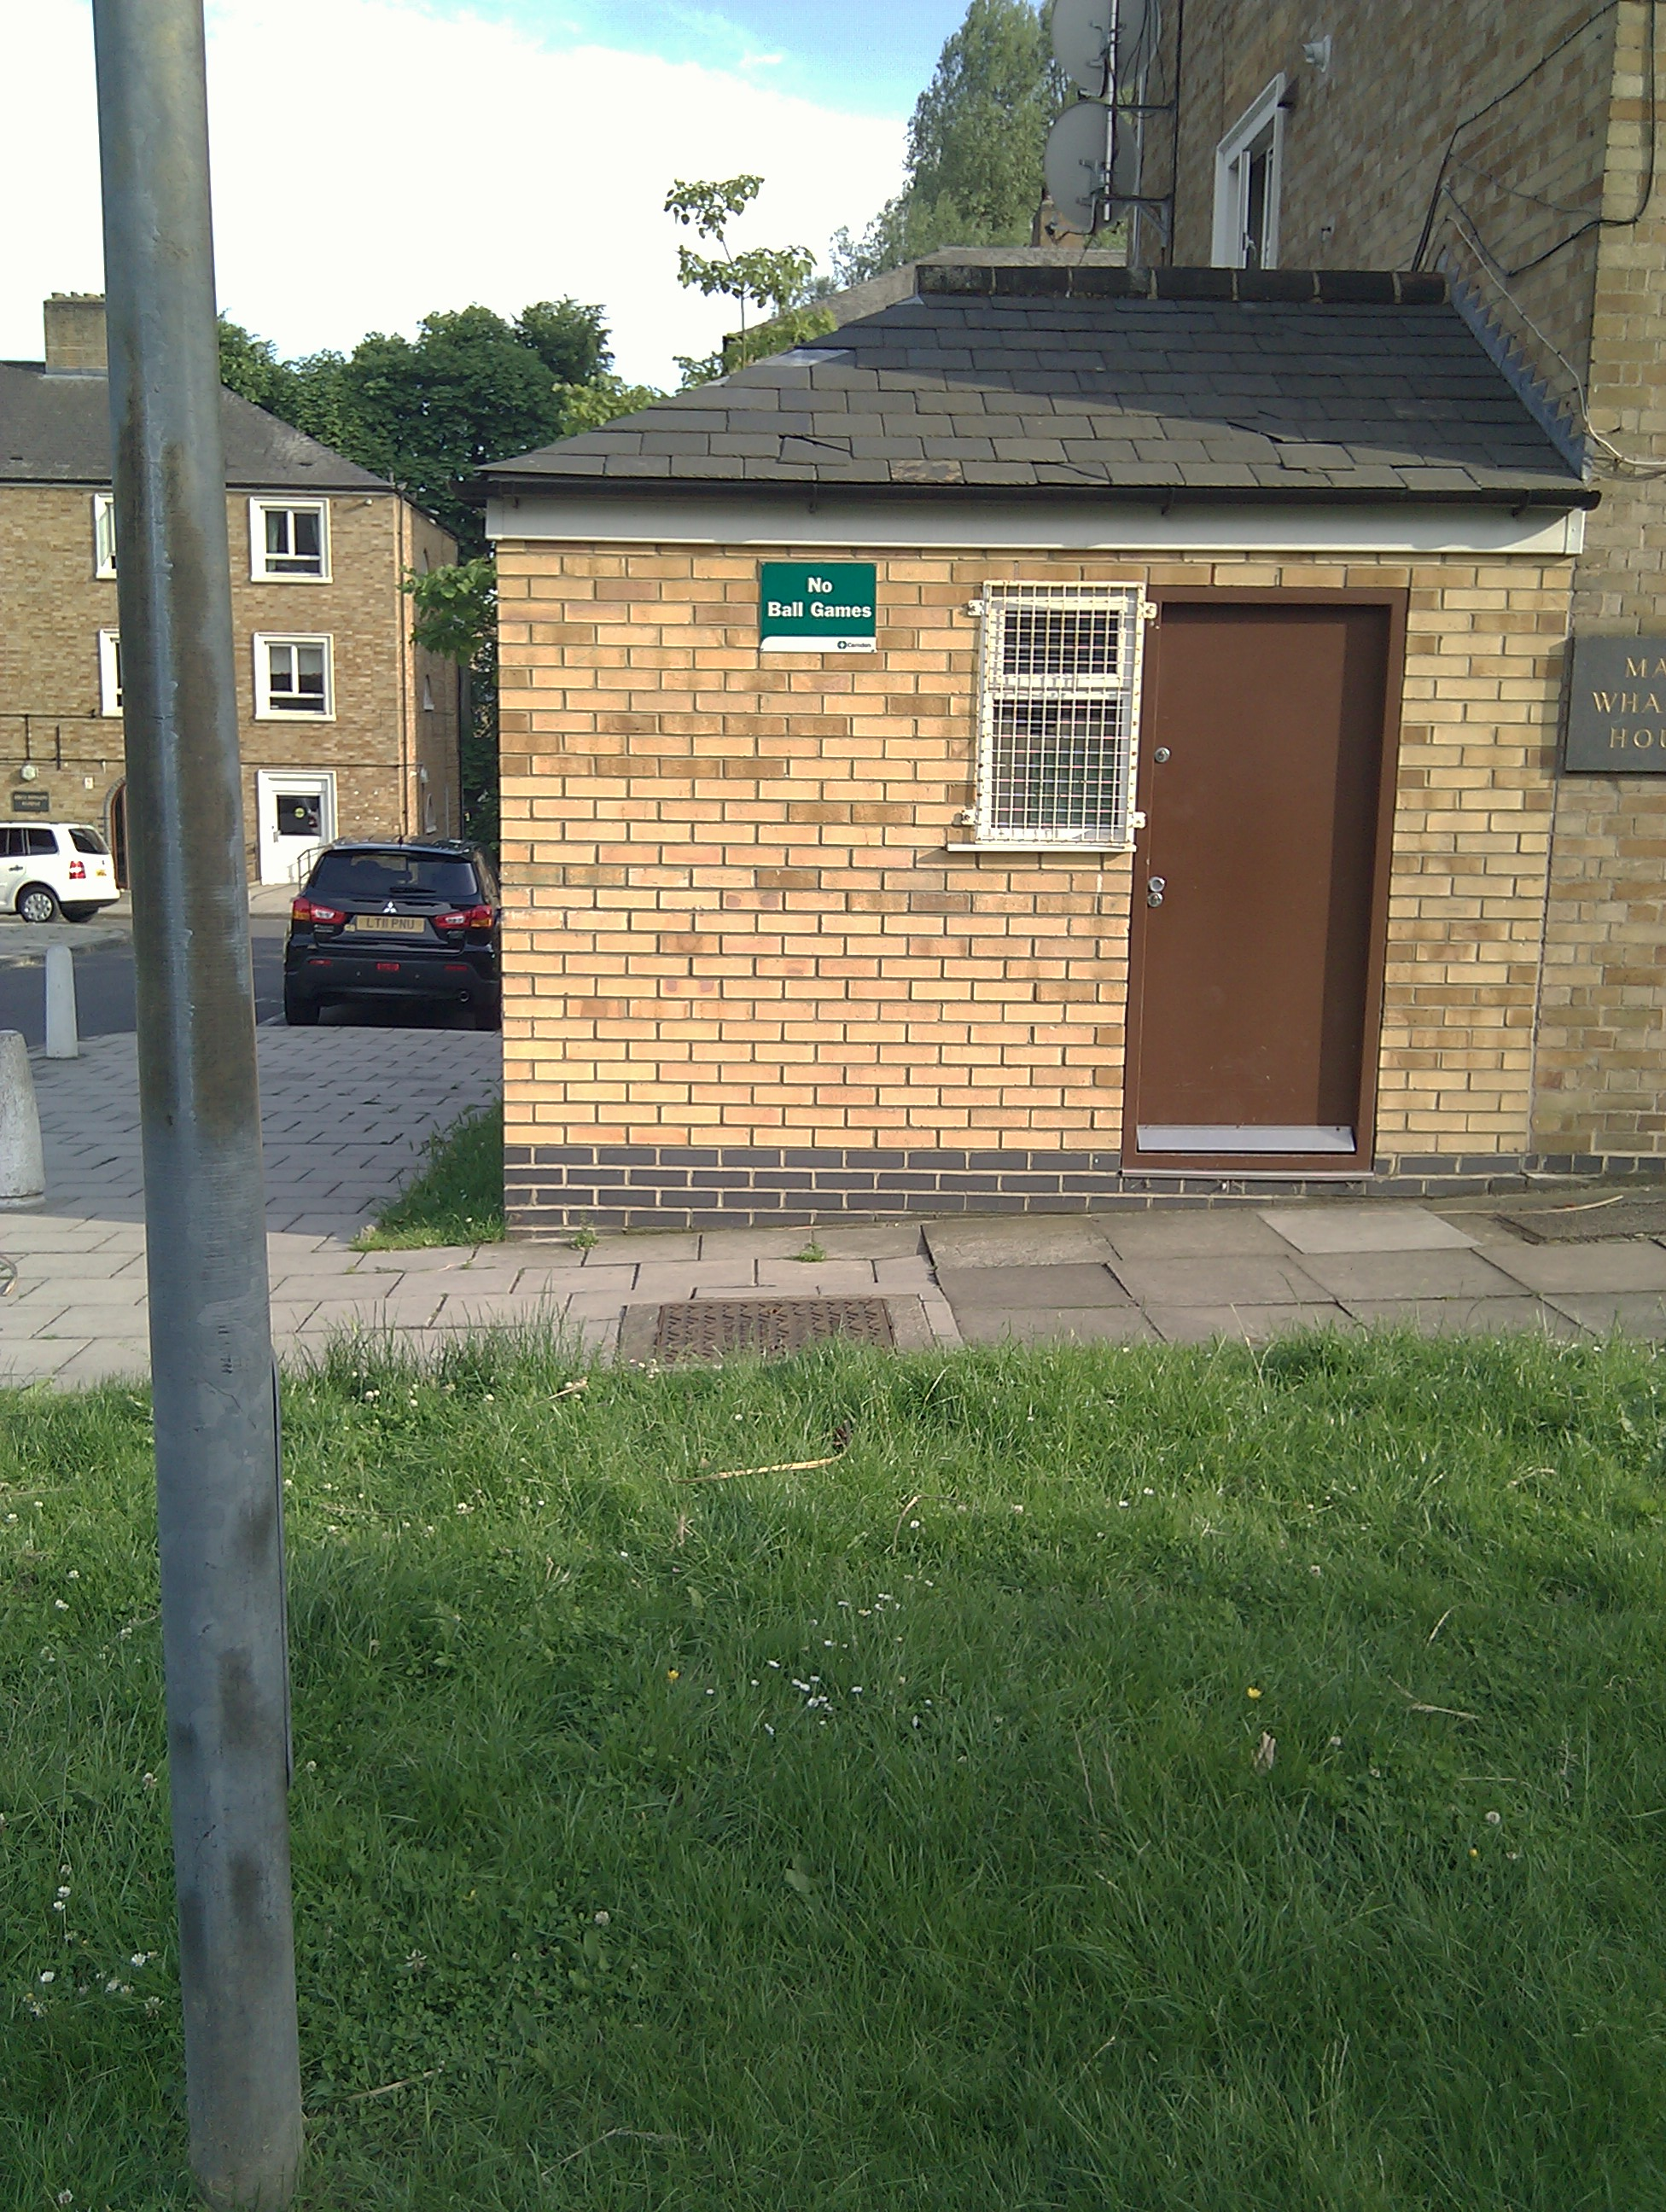
\includegraphics[width=0.35\textwidth]{img/houses1_frame11}  \label{fig:}
 }
 \caption{Example frames for chess and houses1 dataset (used for SfM tools comparison).}
 \label{fig:sfmcomparison0}
\end{figure}

\begin{figure}[htb!]
 \centering
 \subfigure[Bundler output]{
  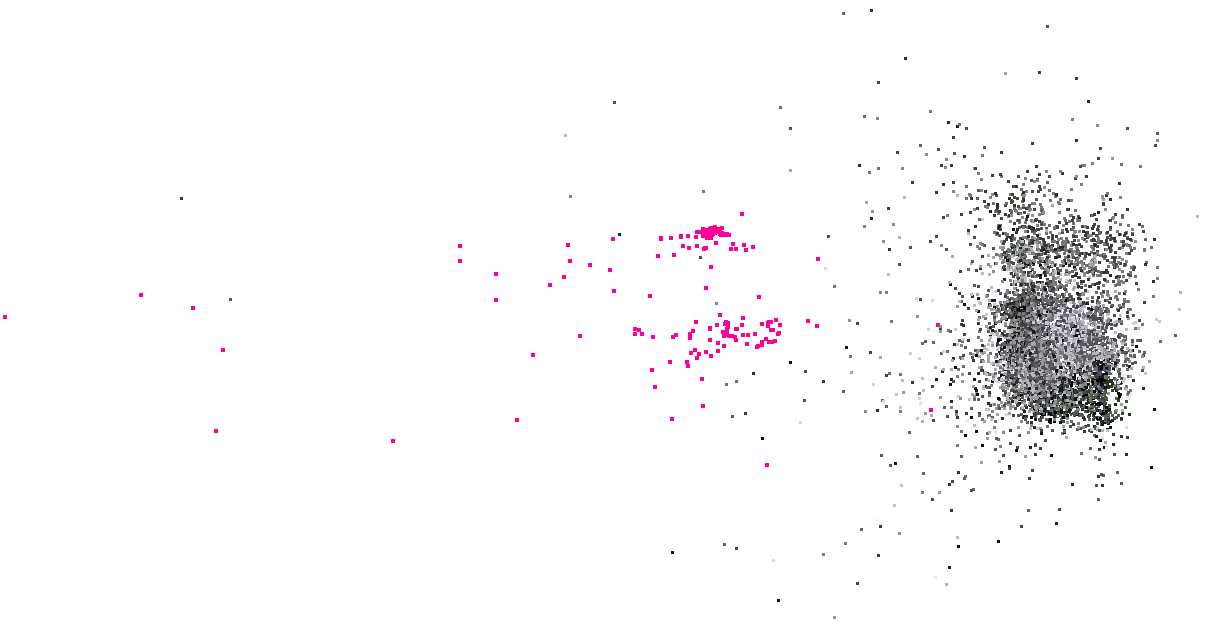
\includegraphics[width=0.9\textwidth]{img/chess_bundler}  \label{fig:}
 }
 \subfigure[Voodoo output]{
  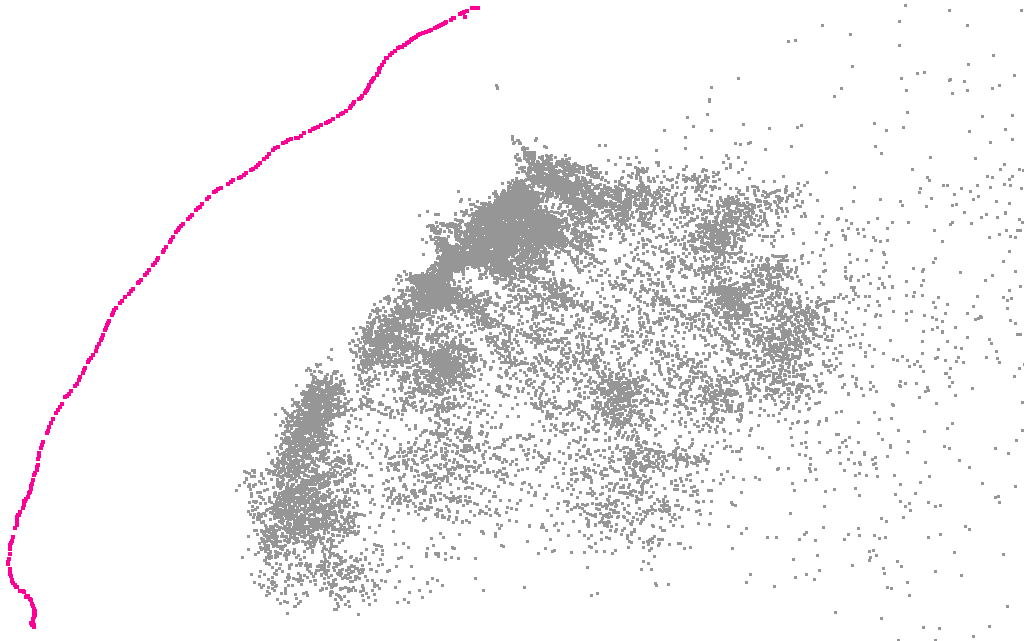
\includegraphics[width=0.9\textwidth]{img/chess_voodoo}  \label{fig:}
 }
 \subfigure[VisualSfM output]{
  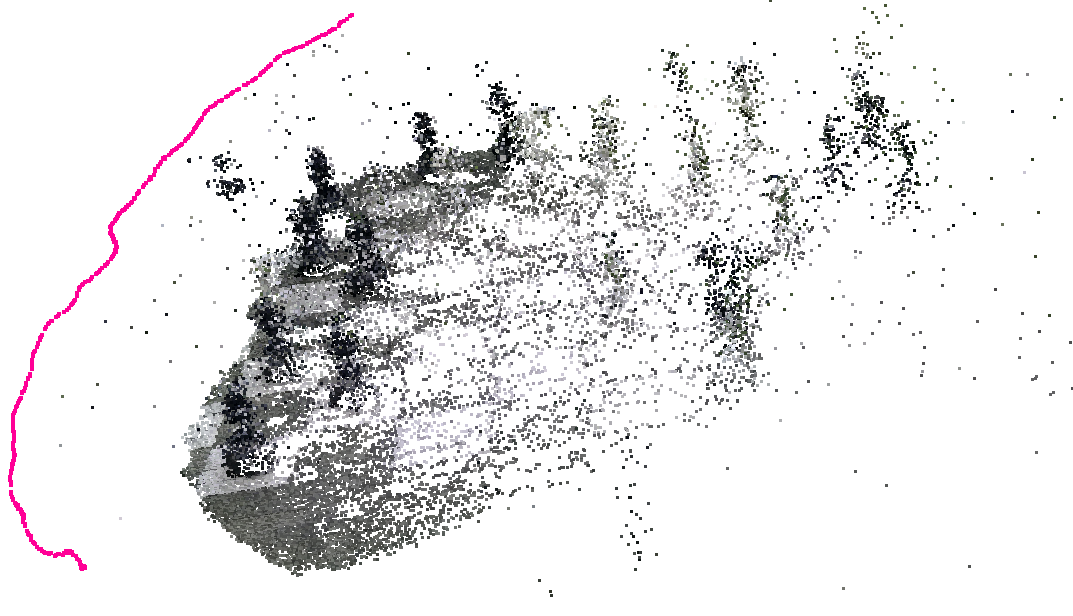
\includegraphics[width=0.9\textwidth]{img/chess_visualsfm}  \label{fig:}
 }
 \caption{Comparison of Structure from Motion tools Bundler, Voodoo and VisualSfM; typical example (chess dataset). Points shown in estimated colour (or grey if not given), camera poses displayed in pink. Visualisations by \texttt{sfmviewer}.}
 \label{fig:sfmcomparison1}
\end{figure}

\begin{figure}[htb!]
 \centering
 \subfigure[Bundler output]{
  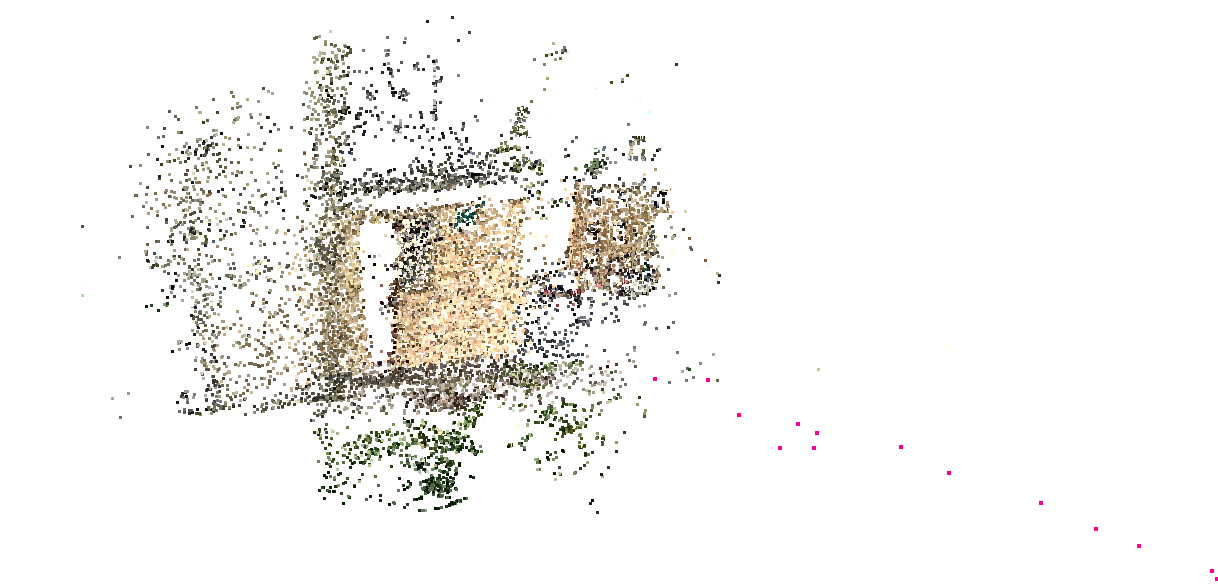
\includegraphics[width=0.9\textwidth]{img/houses1_bundler}  \label{fig:}
 }
 \subfigure[Voodoo output]{
  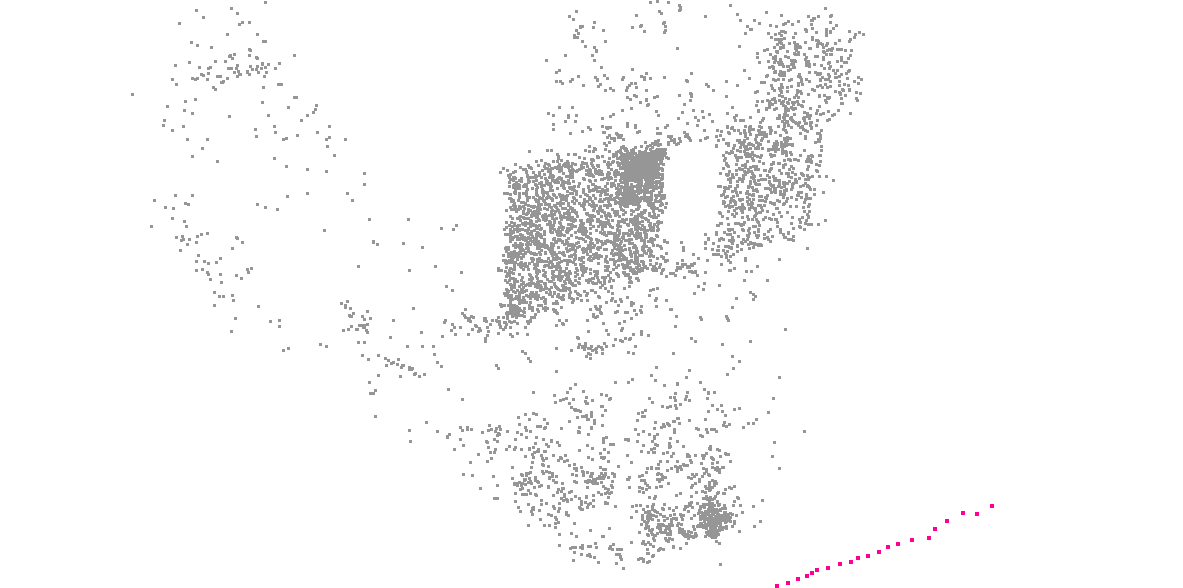
\includegraphics[width=0.9\textwidth]{img/houses1_voodoo}  \label{fig:}
 }
 \subfigure[VisualSfM output]{
  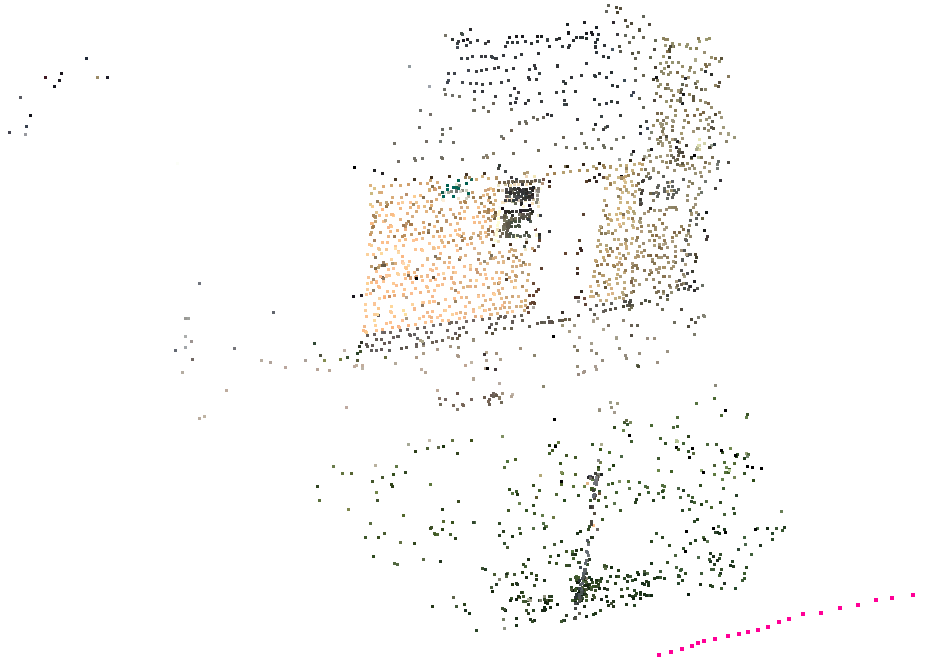
\includegraphics[width=0.9\textwidth]{img/houses1_visualsfm}  \label{fig:}
 }
 \caption{Comparison of Structure from Motion tools Bundler, Voodoo and VisualSfM. Good example (houses1 dataset). Points shown in estimated colour (or grey if not given), camera poses displayed in pink. Visualisations by \texttt{sfmviewer}.}
 \label{fig:sfmcomparison2}
\end{figure}

%   - (reading SfM tools output)
\clearpage
\subsubsection{Reading SfM output}
A common interface class \texttt{sfm\_reader} has been written for reading the various different formats used by different SfM tools. Furthermore, data structures from the C++ standard library are used to represent visibility information. Another reason to discuss this particular class is that it also provides useful methods for the carving algorithm concerning visibility and occlusion.

Four file formats parsers are written. The ply format (Stanford) is shared among SfM tools; however, it only contains points or polygon meshes. Ply files consist of a table (therefore, no variable length lists can be represented) and data can be binary or ASCII. The binary variant can be read by the PCL library, but for the ASCII data variant a parser has been written. Bundler and VisualSfM can both output the ASCII ply format, and VisualSfM outputs the binary ply format after dense reconstruction with CMVS/PMVS. Voodoo can output scripts for various programs (such as Blender). Its native output format has the common extension .txt and contains a list of points and a list of camera models.  Bundler's native output format has extension .out and contains camera models, points, and a visibility list for each point. VisualSfM's native output format has extension .nvm and contains the same information as Bundler's, although it contains a different camera model using quaternions instead of $R, t$ matrices, and distortion has one parameter instead of two. For all three native formats a parser have been written.

Points are saved in a \texttt{PointCloud} object as provided by PCL. It uses \texttt{PointXYZRGB} points which contain a location and an RGB colour. Cameras are saved in two separate structures: camera poses are saved in another \texttt{PointCloud} for easy visualisation - no pyramid-like camera visualisation wrappers are provided by PCL - as well as in a separate list of \texttt{camera} structures. The user-defined \texttt{camera} structure contains intrinsics $R$ and $t$, focal length, and two radial distortion parameters. All camera models from the different file formats are converted to this structure (\eg quaternion to $R$ matrix). Each visibility list is saved in a \texttt{std::map} object mapping every frame index for which a point was detected to a \texttt{visibility} structure. This user-defined structure contains the index of the feature for the particular frame, and the x and y coordinate of detection in the frame. Every feature point now has a global $(x,y,z)$ position in the \texttt{PointCloud} object, and a list of local $(x,y)$ camera coordinates for those cameras that detected the feature point. The map object allows for fast checks on visibility given a frame and feature point number, even for larger sets of frames.

Class \texttt{sfm\_reader} provides re-projection methods for given feature point and camera, including re-distortion. The method \texttt{reprojectsInsideImage} returns a boolean indicating whether a given point re-projects inside a camera window or not. This method is also used by \texttt{selectPointsForCamera}, which re-projects all points inside a given camera and makes an occlusion list of those points that could have been visible, but have not been detected (\ie the camera is not present in the visibility list). A list of currently visible points is made as well.

%   - (extending vis lists)
\subsection{Extending visibility lists}
The optional step of extending visibility lists checks all point-camera pairs that are not represented yet in the vector of maps of visibility information. In practise, this is implemented by looping through the points and, for each point, creating a visibility and invisibility list with help of the re-projection functions. Then, the whole sequence of a particular point is followed and all invisibility entries (re-projects inside image but not detected) are checked. The check consists of finding the nearest camera in absolute distance that did detect the feature point, re-projecting the point into that image and the current image, and comparing patches around the points. The size of the patches is determined by translating the feature point half the size of a voxel (given by the octree) in a direction perpendicular to the vector between the point and camera pose, re-projecting the translated point into one of the images, and calculating the distance to the projection of the original point. This distance is an approximation of the size of a projected voxel near the feature point, and is used to extract rectangular patches from the two images. They are compared by calculating the mean squared distance. A value below the threshold causes the camera index to be added to the visibility list of the feature point. By manually inspecting patch pairs and mean squared distance values, the threshold was set to 0.2 for all further experiments.

%   - carving
\subsection{Carving}
The proposed carving algorithms are implemented using the probabilistic octree of the OctoMap library \cite{Wurm2010}. The octree is initialised with a single parameter specifying the smallest node size possible. By default, all ray shooting operations are executed on nodes at this smallest scale, that is, the leaf nodes in the tree representation. Various node types are provided, the one containing probabilities is used. Probabilities are stored logarithmically, but conversion to and from normal probability values is straight-forward. Two thresholds are used to allow nodes to be labelled with either `free' ($val <= Thr_{free}$) or `occupied' ($val >= Thr_{occ}$), or no label (unknown). Those thresholds are $Thr_{free} = 0.2$ and $Thr_{occ} = 0.7$ by default, and are kept at these values for all experiments. For memory efficiency, eight (leaf) nodes can be merged recursively if they have the same label, thereby averaging and thus losing individual occupancy probabilities. By default leaf nodes are not initialised and depth of the tree is kept to a minimum.

For the implemented space carving algorithms, the octree is initialised with smallest node size equal to the largest axis variation in the feature point \texttt{PointCloud} divided by a given resolution parameter. OctoMap provides two ray shooting methods: \texttt{computeRayKeys} takes as input two points and returns a list of node keys that were hit by the ray between the two points; \texttt{insertRay} does the same, but sets the last node to $Thr_{occ}$ and all the others to $Thr_{free}$ instead of returning the list. The latter is used for the binary Visibility Space Carving algorithm (Alg. \ref{alg:vis-carving}), and the former is used for both probabilistic Visibility-Occlusion Space Carving algorithms (Alg. \ref{alg:vis-occ-carving} and \ref{alg:vis-occ-carving-veto}), there where \texttt{getVoxelsBetween} is mentioned. Note that since we carve tubes of space in this implementation, the resolution parameter potentially has a big influence on the result. In practise, there is a range of possible resolution values that give good results, and the range is laid down by the dataset provided.

%   - regularisation
\subsection{Regularisation}
Regularisation is implemented used the code provided by \Boykov2004. For simplicity, the octree is converted to a voxel grid with voxels the size of the smallest possible octree node. First an empty voxel grid is initialised using the occupancy prior for unknown space, which we set to $Thr_{unknown} = 0.2$. Since conversion splits existing bigger nodes and adds nodes where nothing was initialised before, this increases memory usage quite a lot. This means that only lower resolution settings can be used in the regularisation process. After applying the graph-cut algorithm the voxel grid is converted back to the memory-efficient octree representation.

%   - visualisation/viewers:
\subsection{Visualisation}
During the pipeline, a few intermediate and final results can be visualised. Three visualisation tools are developed and one provided by the OctoMap library is used. We will discuss each briefly. The first two tools are used for visualising features before carving, one 2D image annotator and one interactive 3D tool. The two other tools are meant for visualising voxel grids after carving, again one 2D image annotator and one interactive 3D tool.

%     - features (annotated imgs)
Although external structure from motion tools are being used, a tool has been written for experiments with and visualisations of various feature detectors. It can be used to check the amount of interest points discoverable in a dataset, and the uniqueness of their descriptors during tracking. It is not used in the final pipeline, but is discussed for completeness. The visualiser, \texttt{featureviewer}, takes as input either a video, directory with images, or webcam stream, and annotates the images with a given type of interest point (\eg SIFT, SURF, ORB, FAST, HARRIS) including their size, plus edges (Canny edge-detector). One can interactively click on a feature point, which will be matched over the sequence by a simple ratio test: if the ratio of the two best matches in the next or previous frame (\ie the L1 distance) is big, the interest point is quite unique and the best match is taken. If the ratio is close to 1, we keep the last known good descriptor and continue to the next frame. Note that this simple heuristic does not use any location prior. We can define the visibility confidence as one minus that ratio, and plot it for the sequence, similar to the visibility tracks shown in Fig. \ref{fig:vis-carving} and \ref{fig:vis-occ-carving}. One example image processed with \texttt{featureviewer} is shown in Figure \ref{fig:featureviewer}.

%     - sfm (3D)
Visualisation of triangulated SfM feature points or dense point clouds can be done with \texttt{sfmviewer}. The SfM tools outputs (Fig. \ref{fig:sfmcomparison1} and \ref{fig:sfmcomparison2}) were made this way. It uses class \texttt{sfm\_reader} for opening SfM output files and representing their contents. The PCL library provides wrappers around the VTK visualisation toolkit. It is used for easy point cloud visualisation, both the feature point cloud and camera poses. Interaction is implemented using the default PCL visualiser for mouse navigation, plus VTK call-back functions for custom shortcuts, and selection of points and cameras. Selecting a point colours the cameras that detected the point (using the visibility list of the point). Selecting a camera calls \texttt{selectPointsForCamera} as described earlier, thereby projecting all the points into the camera. Detected points are coloured green, while undetected points that do re-project within the image borders but are coloured red. To be able to recover the original point colours during the next selection, \texttt{sfm\_reader} keeps a shadow copy of the original point cloud. Another implemented feature is the ability to visualise those visible (green) and invisible (red) points onto the original corresponding frame. The camera-feature pairs can be visualised even more explicitly by drawing green lines between the camera and visible points or between the point and detecting cameras. Two example visualisation is shown in Fig. \ref{fig:sfmviewer1} and \ref{fig:sfmviewer2}.

\begin{figure}[htb!]
 \centering
 \subfigure[\texttt{featureviewer} for frame in chess, including SIFT features and visibility track for the green interest point]{
  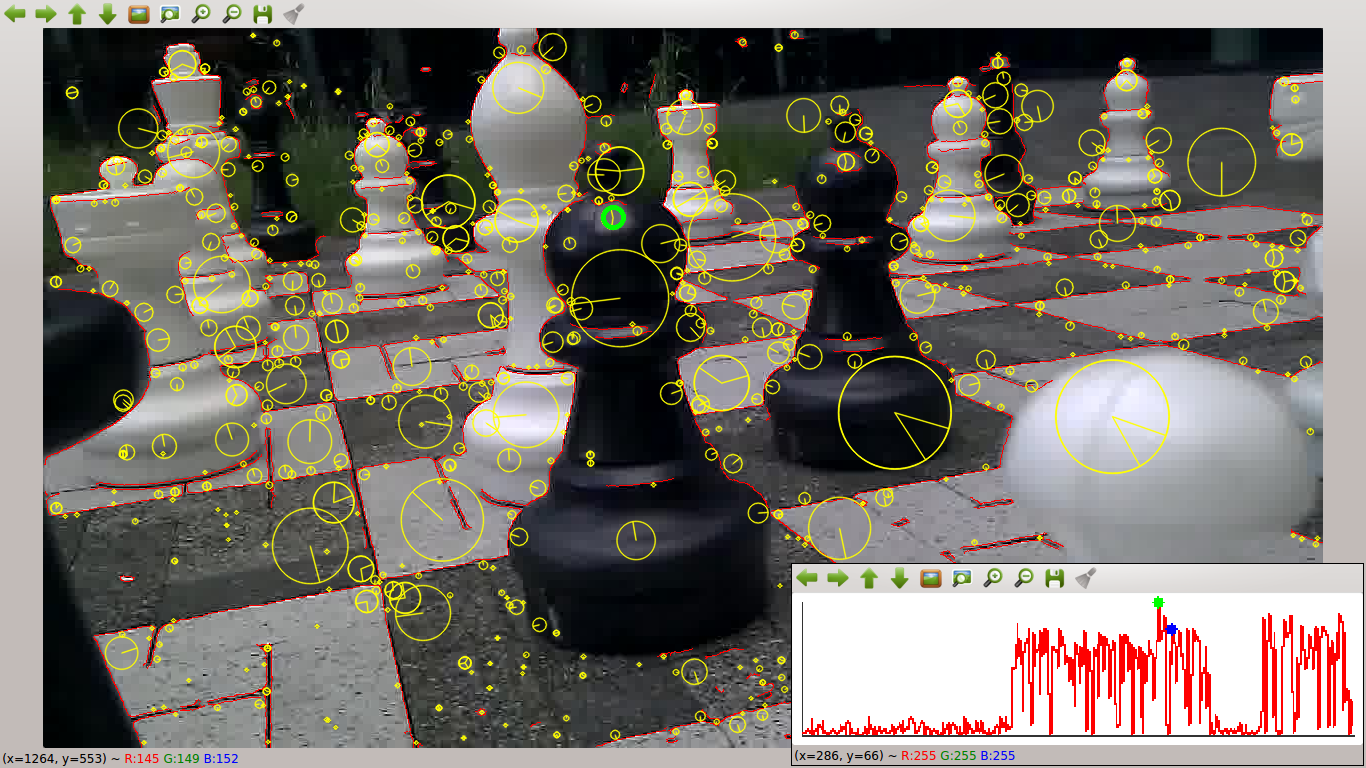
\includegraphics[width=0.9\textwidth]{img/featureviewer}  \label{fig:featureviewer}
 }
 \subfigure[\texttt{sfmviewer} for selected camera of lampposts\_on\_wall1; one lamppost causes a red area to emerge on the wall, but the conservative visibility information of VisualSfM is noticeable too in the `green' areas]{
  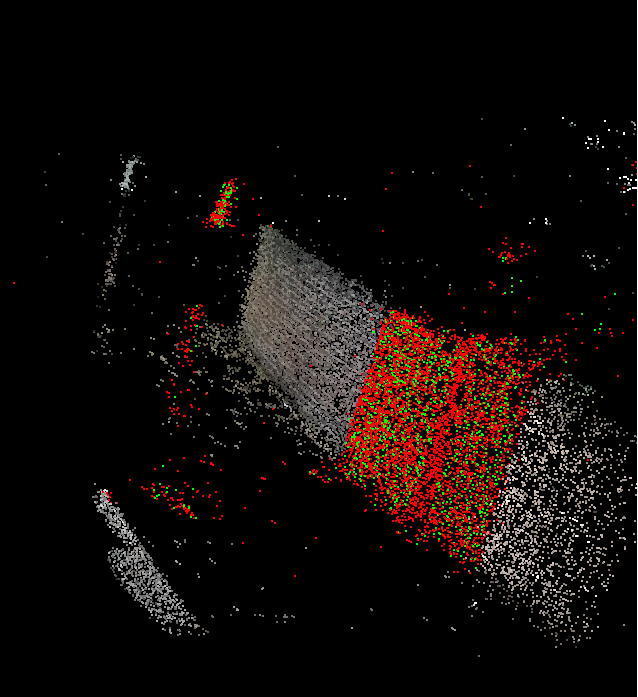
\includegraphics[width=0.45\textwidth]{img/sfmviewer2}  \label{fig:sfmviewer1}
 }
 \subfigure[\texttt{sfmviewer} for selected point of sainsburys1; two reflective poles become `visible' due to absence of lines]{
  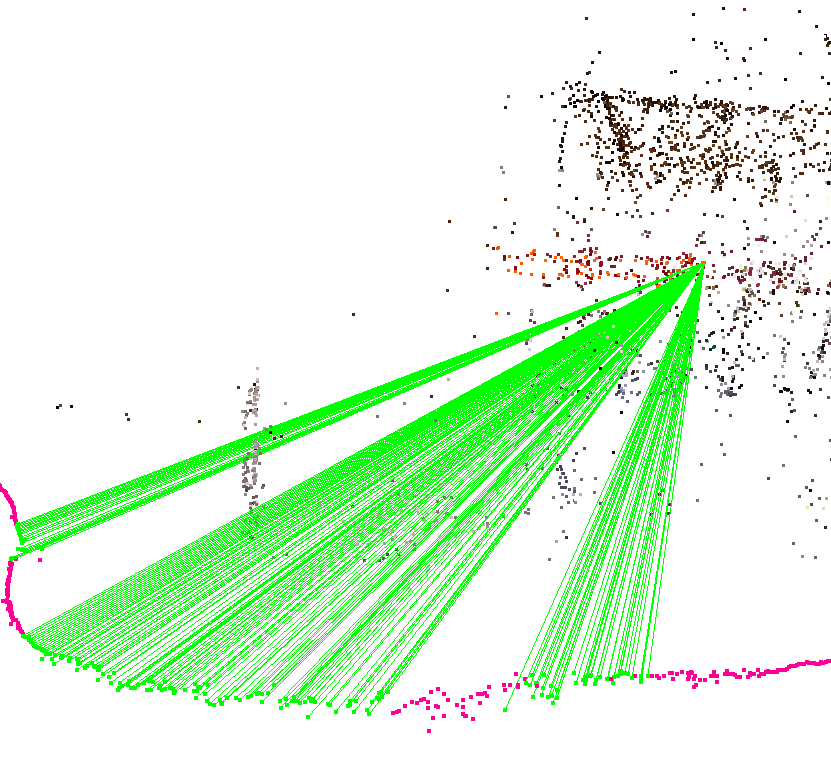
\includegraphics[width=0.45\textwidth]{img/sfmviewer1}  \label{fig:sfmviewer2}
 }
 \subfigure[\texttt{carveviewer} for frame in sciencepark2 (with incorrect nearby voxels at the top and only few detected features)]{
  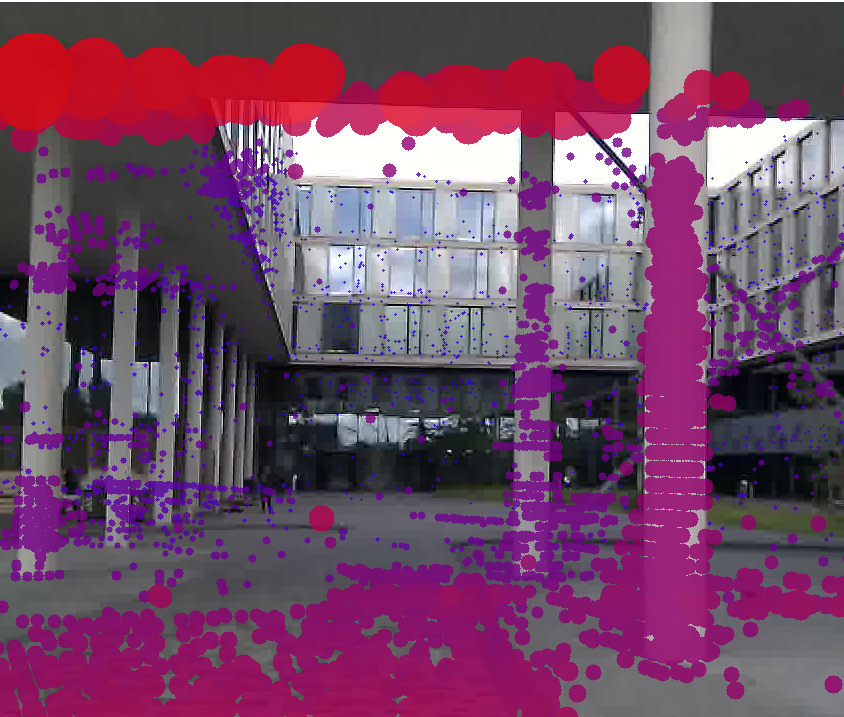
\includegraphics[width=0.45\textwidth]{img/carveviewer}  \label{fig:carveviewer}
 }
 \subfigure[\texttt{octovis} view for houses1; a partly reconstructed lamppost is visible on the left (purple)]{
  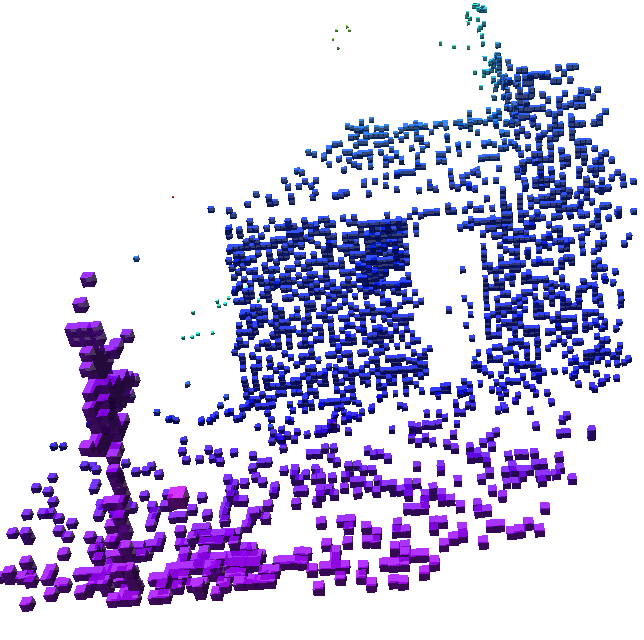
\includegraphics[width=0.45\textwidth]{img/octovis}  \label{fig:octovis}
 }
 \caption{Visualisations by three developed tools and one provided viewer}
 \label{fig:visualisationtools}
\end{figure}

\clearpage
%     - carveviewer (annotated imgs)
After space carving has been done, a probabilistic octree is the result. For visualisation purposes, we use the occupancy threshold $Thr_{occ}$ to make a binary distinction between occupied and not occupied. The last developed visualisation tool, \texttt{carveviewer}, annotates the original images with the carved octree. To prevent axis dependent results, all nodes are imagined as spheres and projected on top of the images. As with the code for extending visibility lists, both the node centres and centres with offsets the size of the nodes are projected into the images, and the projected points are used to estimate the radii, resulting in a list of $x,y,r$ entries. Then, rays are casted from the camera in the direction of the projected nodes, and all rays hitting another, occluding node before the projected one, are removed from the list. The remaining nodes are visible from the given camera and are drawn as semi-transparent circles on top of the image. The circles are drawn with the estimated radii and coloured according to the log distance from the camera (nearby voxels are red, voxels far away blue). One example rendering is shown in Figure \ref{fig:carveviewer}. For more dense voxel grids, results remind of depth maps on top of their original images. 

%     - octovis (3D)
An interactive octree viewer is provided by the OctoMap library. It has been used without modification. Nodes are rendered as semi-transparent cubes which are either light blue for occupied and dark blue for very high occupancy probability (threshold undefined), or coloured according to the value of one of the axes. Optionally, free space (occupancy probability below $Thr_{free}$) can be visualised too as green cubes. One example view is shown in Figure \ref{fig:octovis}.

The visualisation tools will be used extensively in the next chapter.

